\ifx\wholebook\relax \else
% ------------------------

\documentclass[b5paper]{article}
\usepackage[nomarginpar
  %, margin=.5in
]{geometry}

\addtolength{\oddsidemargin}{-0.05in}
\addtolength{\evensidemargin}{-0.05in}
\addtolength{\textwidth}{0.1in}
\usepackage[en]{../../../prelude}

\setcounter{page}{1}

\begin{document}

\title{Binary Heaps}

\author{Xinyu LIU
\thanks{{\bfseries Xinyu LIU} \newline
  Email: liuxinyu95@gmail.com \newline}
  }

\maketitle
\fi

\markboth{Binary Heaps}{Elementary Algorithms}

\ifx\wholebook\relax
\chapter{Binary Heaps}
\numberwithin{Exercise}{chapter}
\fi

\section{Definition}
\label{introduction} \index{Binary heap}

Heaps are widely used for sorting, priority scheduling and graph algorithms, and etc.\cite{wiki-heap}. The most popular implementation models the heap as a complete binary tree in array\cite{CLRS}. The most efficient heap sort algorithm developed by R.W. Floyd is also based on this method\cite{wiki-heapsort}\cite{rosetta-heapsort}. For the generic heap definition, we can implement with varies data structures but not limit to array. In this chapter, we focus on the heaps implemented with binary trees, including leftist heap, skew heap, and splay heap\cite{okasaki-book}. A heap is either empty, or stores comparable elements that satisfies a property and three operations:

\begin{enumerate}
\item \textbf{The heap property}: the top element is always the minimum;
\item \textbf{Pop}: removes the top element from the heap and maintain the heap property: the new top is still the minimum in the rest;
\item \textbf{Insert}: add a new element to the heap and maintain the heap property;
\item \textbf{Other}: operations like merge also maintain the heap property.
\end{enumerate}

Because elements are comparable, we can also define the heap always keeps the maximum on top. We call the heap with the minimum on top as {\em min-heap}, the maximum on top as {\em max-heap}. When implement heap with a tree, we can put the minimum (or the maximum) in the root. After pop, we remove the root, and rebuild the tree from the sub-trees. We call the heap implemented with binary tree as {\em binary heap}. This chapter gives three types of binary heap.

\section{Binary heap by array}
\label{ibheap} \index{binary heap by array} \index{complete binary tree}

The first implementation is to represent the a complete binary tree with an array. The complete binary tree is `almost' full. The full binary tree of depth $k$ contains $2^k - 1$ nodes. We can number every node top-down, from left to right as 1, 2, ..., $2^k -1$. The node number $i$ in the complete binary tree is located at the same position in the full binary tree. The leaves only appear in the bottom layer, or the second last layer. Figure \ref{fig:tree-array-map} shows a complete binary tree and the array. As the complete binary tree, the $i$-th cell in array corresponds to a node, its parent node maps to the $\lfloor i/2 \rfloor$-th cell; the left sub-tree maps to the $2i$-th cell, and the right sub-tree maps to the $2i + 1$-th cell. If any sub-tree maps to an index out of the array bound, then the sub-tree does not exist (i.e. leaf node). We can define the map as below (index starts from 1):

\begin{figure}[htbp]
\centering
   \includegraphics[scale=0.45]{img/tree-array-map-tree}
   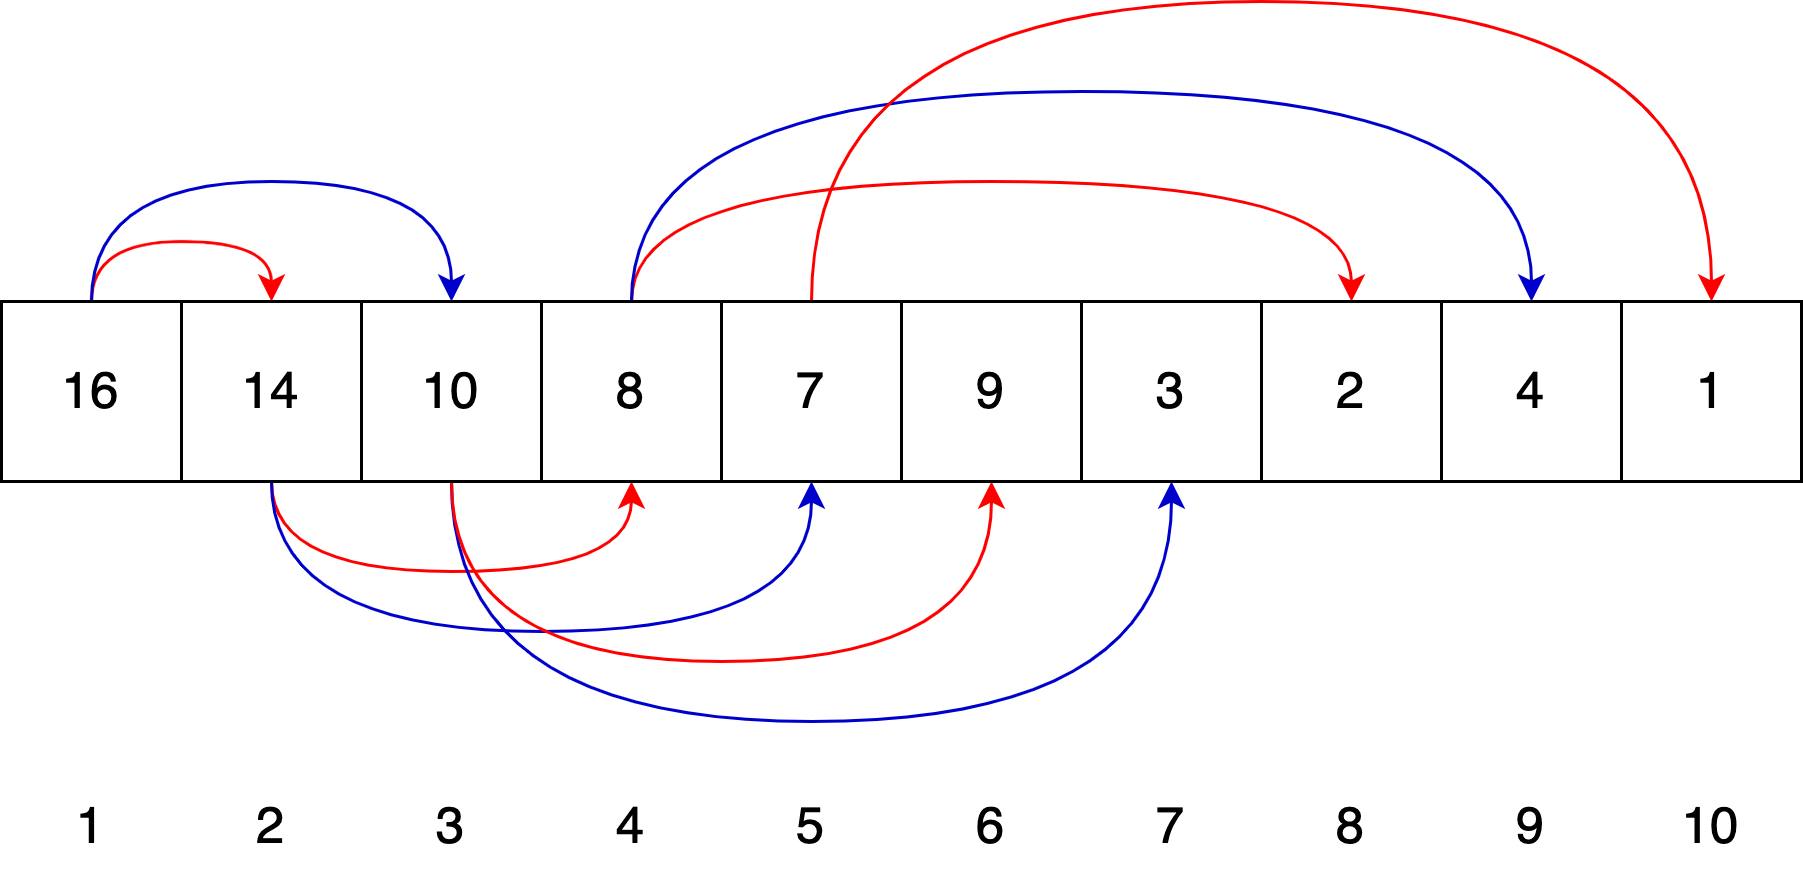
\includegraphics[scale=0.5]{img/binary-tree-in-array}
 \caption{Map between a complete binary tree and an array.} \label{fig:tree-array-map}
\end{figure}

\be
\begin{cases}
parent(i) & = \lfloor \dfrac{i}{2} \rfloor \\
left(i)   & = 2i \\
right(i)  & = 2i + 1 \\
\end{cases}
\ee

\subsection{Heapify}
\index{Binary heap!Heapify}

Heapify is the process maintain heap property, keep the minimum element on the top. For binary heap, we can obtain a stronger property as the binary tree is recursive: every sub-tree stores its minimum element in the root. In other words, every sub-tree is also a binary heap. Consider the min-heap represented with array, for any cell index $i$, we examine if all the elements in sub-trees are greater then or equal to it ($\geq$). Exchange when not satisfies. Repeat this for all sub-trees rooted at $i$.

\begin{algorithmic}[1]
\Function{Heapify}{$A, i$}
  \State $n \gets |A|$
  \Loop
    \State $s \gets i$ \Comment{$s$ is the smallest}
    \State $l \gets$ \Call{Left}{$i$}, $r \gets$ \Call{Right}{$i$}
    \If{$l \leq n$ and $A[l] < A[i]$}
      \State $s \gets l$
    \EndIf
    \If{$r \leq n$ and $A[r] < A[s]$}
      \State $s \gets r$
    \EndIf
    \If{$s \neq i$}
      \State \textproc{Exchange} $A[i] \leftrightarrow A[s]$
      \State $i \gets s$
    \Else
      \State \Return
    \EndIf
  \EndLoop
\EndFunction
\end{algorithmic}

For index $i$ in array $A$, any sub-tree node should not be less than $A[i]$. Otherwise, we exchange $A[i]$ with the smallest one, and recursively check the sub-trees. As the process time is proportion to the height of the tree, \textproc{Heapify} is bound to $O(\lg n)$, where $n$ is the length of the array. Figure \ref{fig:heapify} gives the steps when apply \textproc{Heapify} from $2$ to array [1, 13, 7, 3, 10, 12, 14, 15, 9, 16]. The result is [1, 3, 7, 9, 10, 12, 14, 15, 13, 16].

\begin{figure}[htbp]
  \centering
  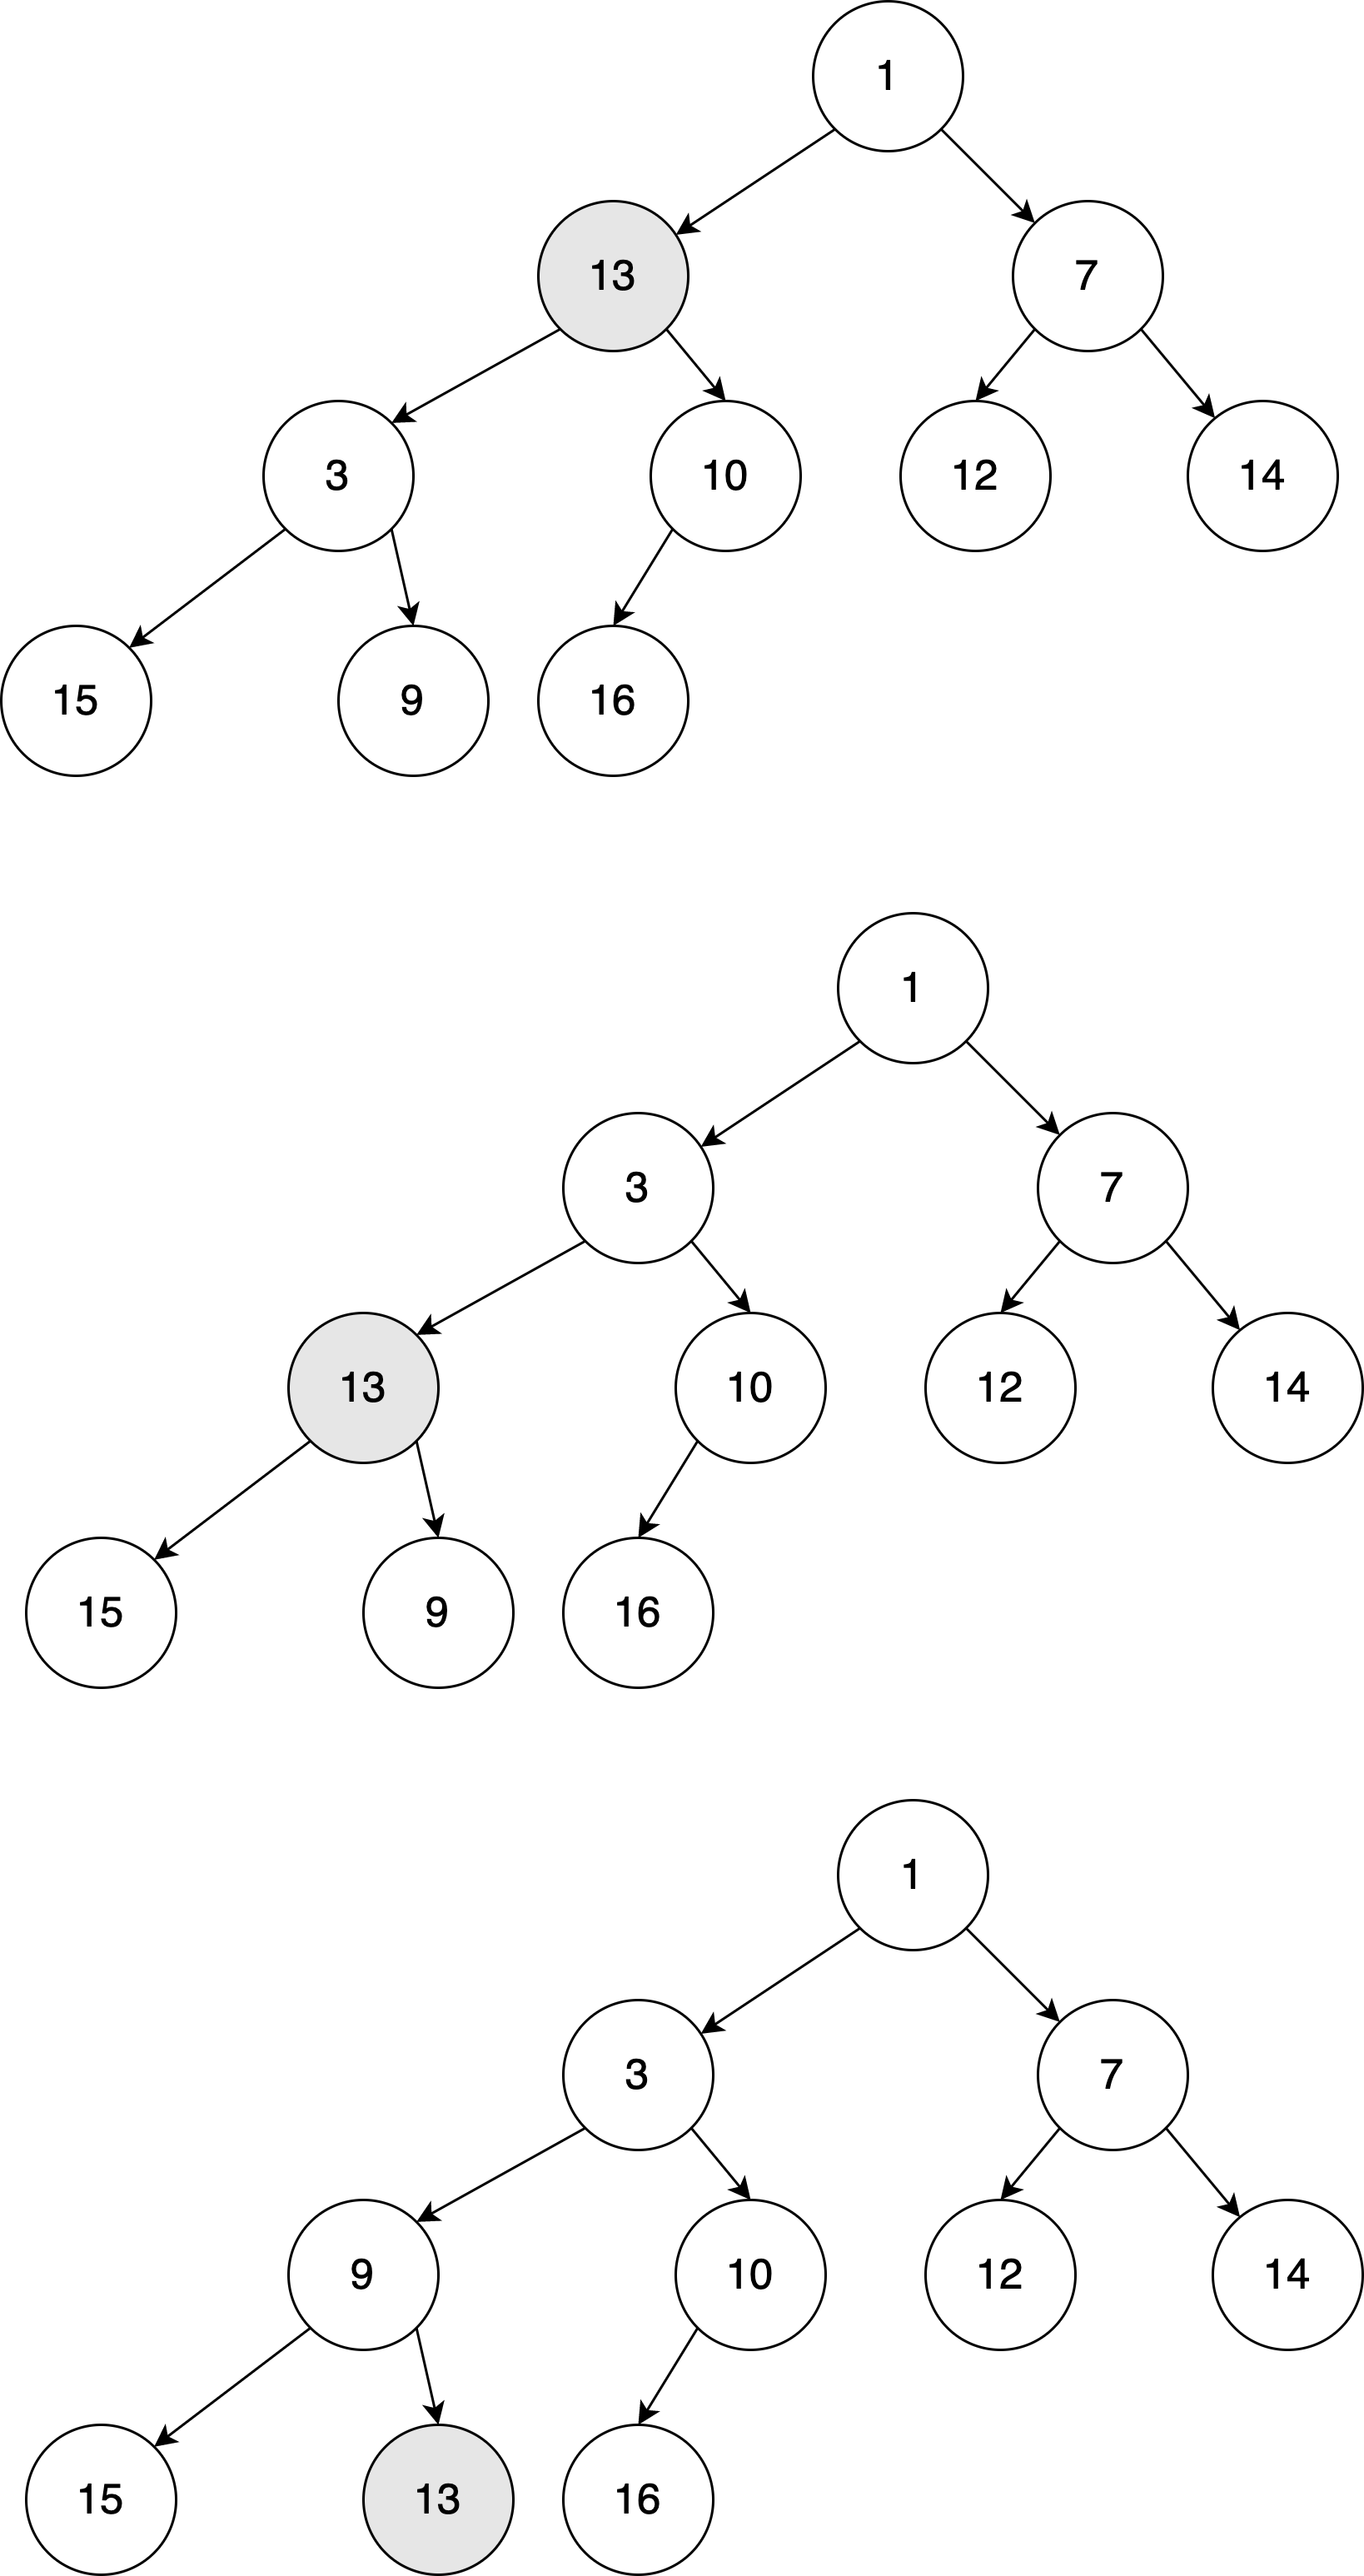
\includegraphics[scale=0.4]{img/heapify}
  \caption{Heapify. Step 1: the minimum of 13, 3, 10 is 3, exchange 3 $\leftrightarrow$ 13; Step 2: the minimum of 13, 15, 9 is 9, exchange 13 $\leftrightarrow$ 9; Step 3: 13 is leaf, terminate.}
  \label{fig:heapify}
\end{figure}

\subsection{Build}
\index{Binary heap!build}

We can build heap from arbitrary array with \textproc{Heapify}. List how many nodes in each level of a complete binary tree: $1, 2, 4, 8, ...$. They are all power of 2 except for the last level. Because the tree is not necessarily full, there are at most $2^{p-1}$ nodes, where $p$ is the smallest integer satisfying $2^p - 1 \geq n$, and $n$ is the length of the array. Skip all leaves because \textproc{Heapify} takes no effect on them, we start applying \textproc{Heapify} to the last branch node (which index $\leq \lfloor n/2 \rfloor$) bottom-up. The build function is defined as below:

\begin{algorithmic}[1]
\Function{Build-Heap}{$A$}
  \State $n \gets |A|$
  \For{$i \gets \lfloor n/2 \rfloor$ down to $1$}
    \State \Call{Heapify}{$A, i$}
  \EndFor
\EndFunction
\end{algorithmic}

Although \textproc{Heapify} is bound $O(\lg n)$ time, \textproc{Build-Heap} is bound to $O(n)$, but not $O(n \lg n)$. We skip all leaves, check and move down a level at most for $1/4$ nodes; check and move down two levels at most for $1/8$ nodes; check and move down three levels at most for $1/16$ nodes... the total comparison and move times is up to:

\be
S = n (\frac{1}{4} + 2 \frac{1}{8} + 3 \frac{1}{16} + ...)
\label{eq:build-heap-1}
\ee

Multiply by 2 for both sides:

\be
2S = n (\frac{1}{2} + 2 \frac{1}{4} + 3 \frac{1}{8} + ...)
\label{eq:build-heap-2}
\ee

Subtract (\ref{eq:build-heap-1}) from (\ref{eq:build-heap-2}):

\bea*{rcll}
2S - S & = & n [\dfrac{1}{2} + (2 \dfrac{1}{4} - \dfrac{1}{4}) + (3 \dfrac{1}{8} - 2 \dfrac{1}{8}) + ...] & \text{shift by one and subtract} \\
     S & = & n [\dfrac{1}{2} + \dfrac{1}{4} + \dfrac{1}{8} + ...] & \text{geometric series} \\
       & = & n
\eea*


Figure \ref{fig:build-heap-3} shows the steps to build a min-heap from array $[4, 1, 3, 2, 16, 9, 10, 14, 8, 7]$. The black node is where \textproc{Heapify} is applied. The grey nodes are swapped to maintain the heap property.

\begin{figure}[htbp]
  \centering
  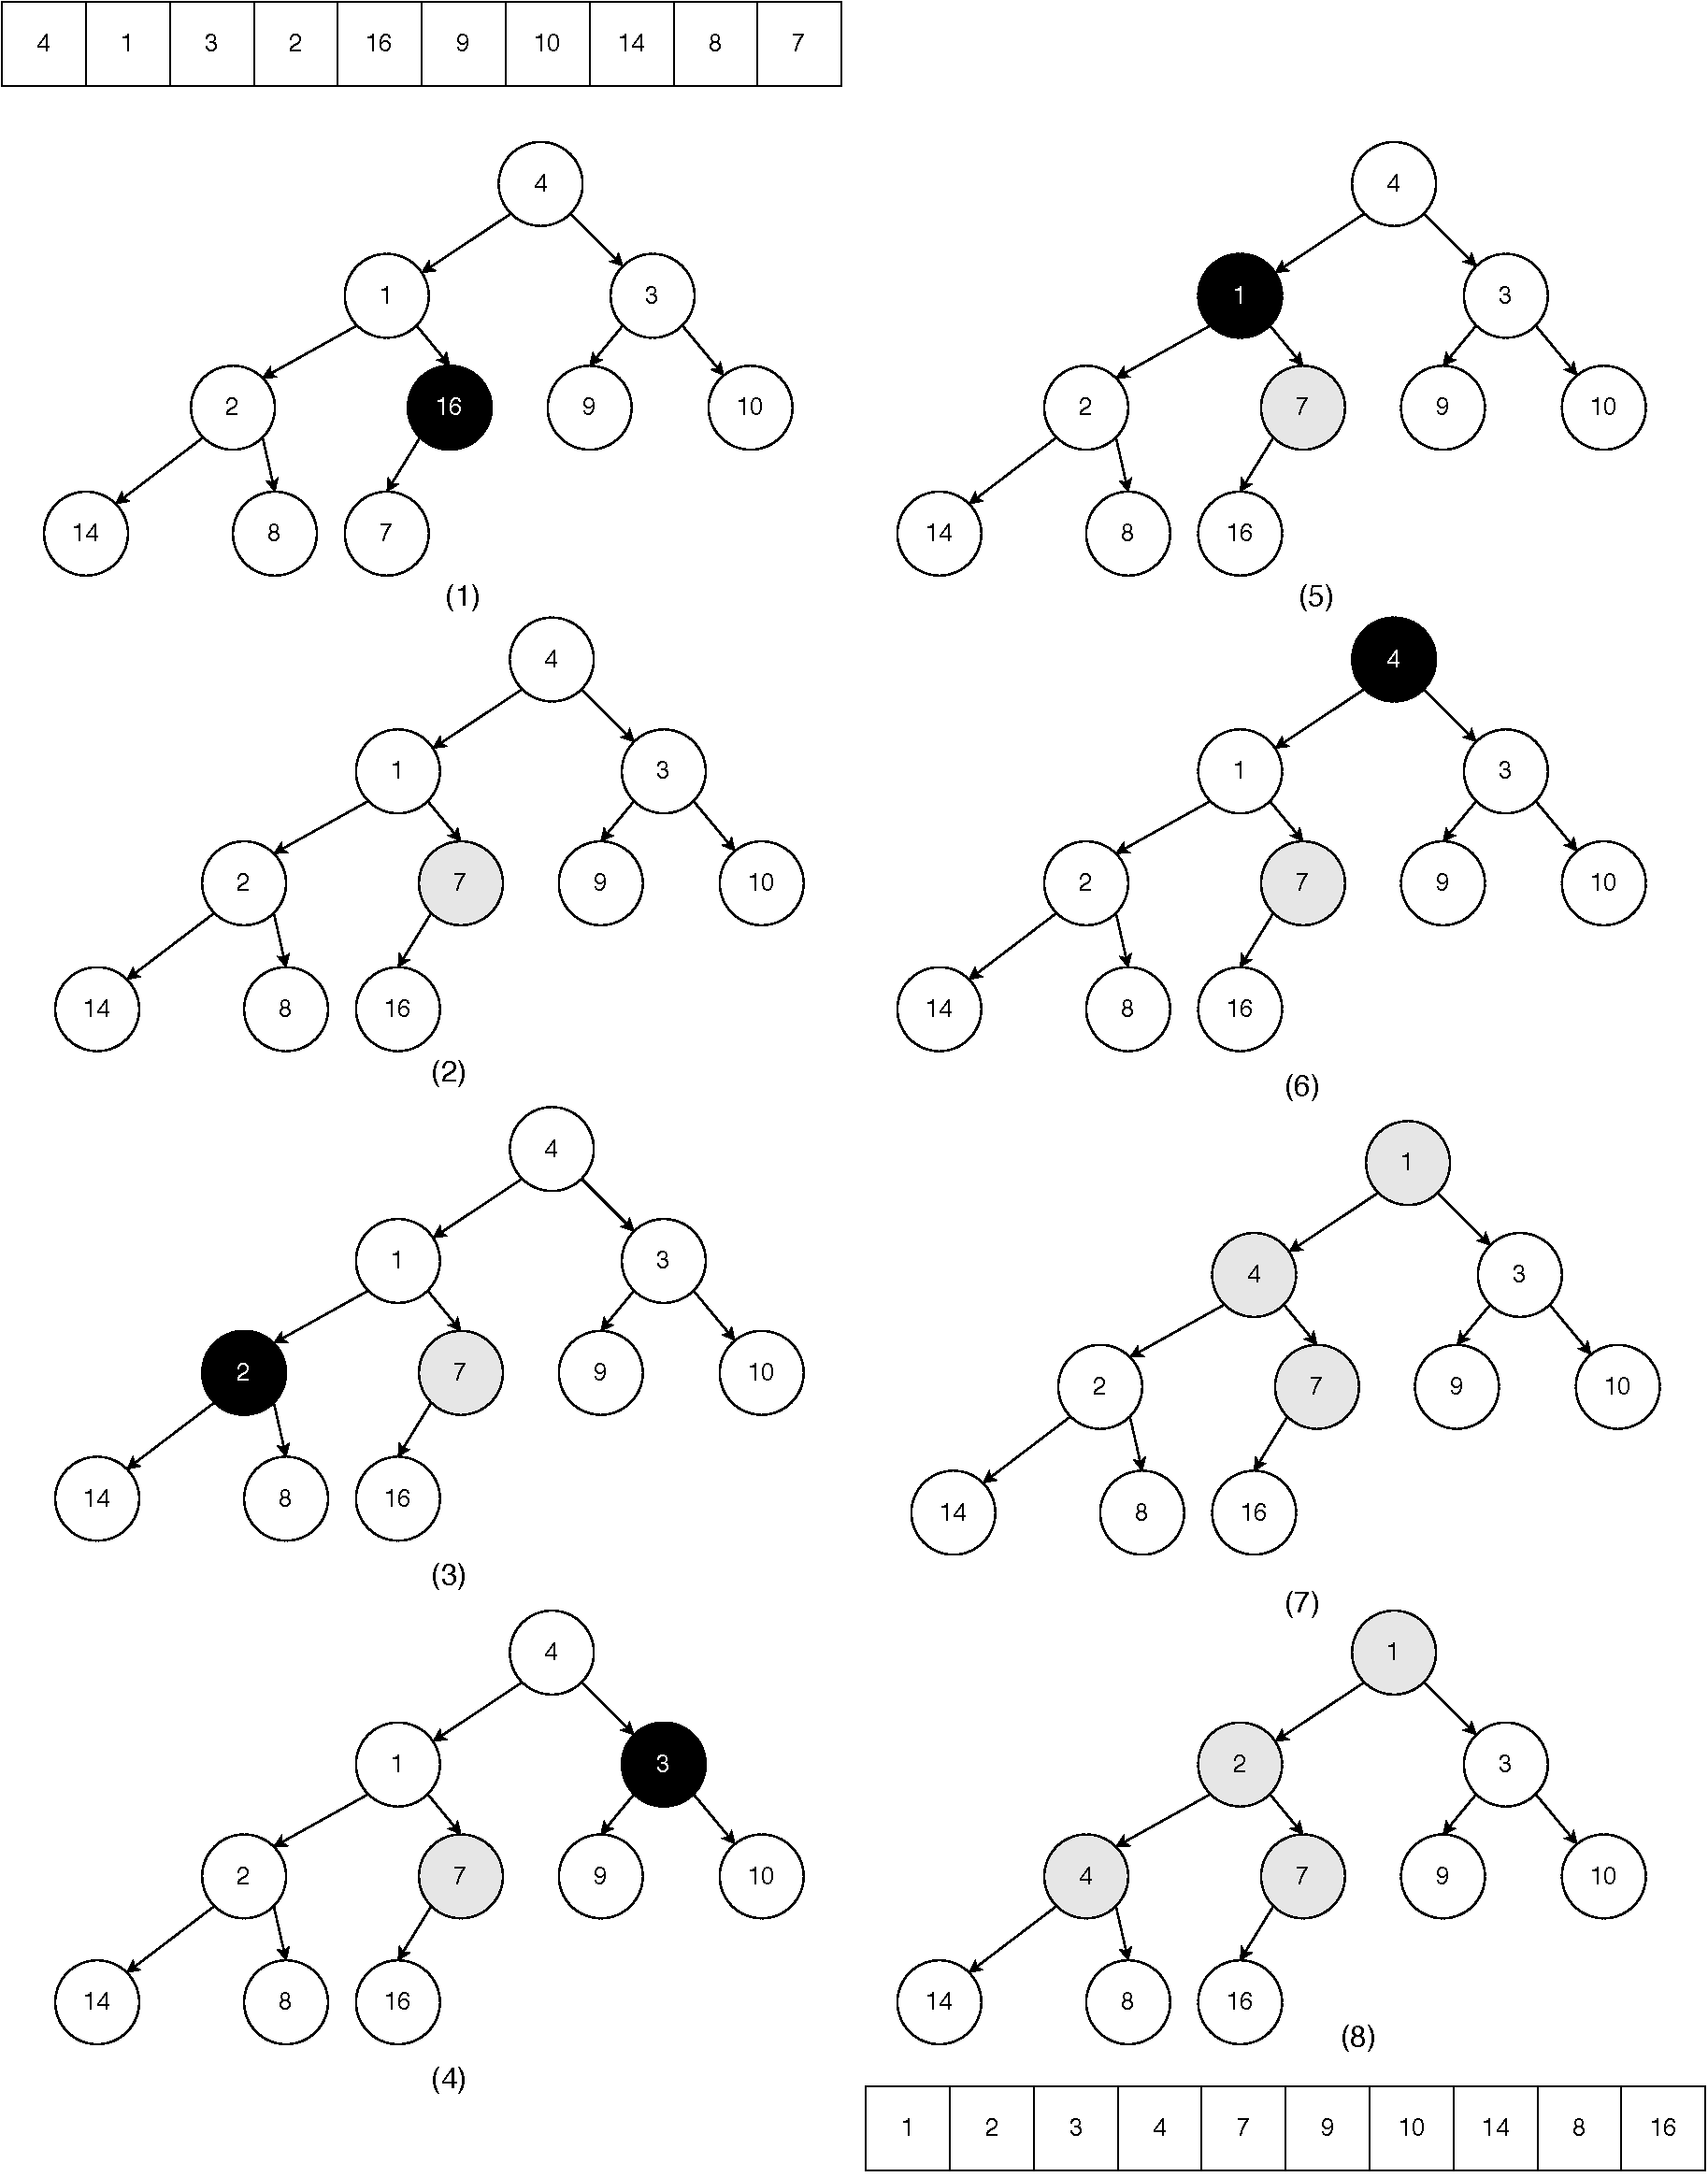
\includegraphics[scale=0.4]{img/build-heap}
  \caption{Build heap. (1) 16 > 7; (2) exchange 16 $\leftrightarrow$ 7; (3) 2 < 14 and 2 < 8; (4) 3 < 9 and 3 < 10; (5) 1 < 2 and 1 < 7; (6) 1 < 4 and 1 < 3; (7) exchange 4 $\leftrightarrow$ 1; (8) exchange 4 $\leftrightarrow$ 2, end.}
  \label{fig:build-heap-3}
\end{figure}

\subsection{Heap operations}

Heap operations include access the top, pop, look up the top $k$ elements, decrease an element in min-heap (or increase an element in max-heap), and insert a new element. For binary heap, the root stores the minimum element, corresponding to the first cell in array:

\index{Binary heap!top}
\begin{algorithmic}[1]
\Function{Top}{$A$}
  \State \Return $A[1]$
\EndFunction
\end{algorithmic}

\subsubsection{Pop}
\index{Binary heap!pop}

After pop, the remaining elements in array shift ahead by one. However, after removed the root of the binary tree, the rest is not a binary tree any more. To avoid such situation, we swap the first and the last element in array, then reduce the array length by one. It equivalent to remove a leaf but not the root. We then apply \textproc{Heapify} to recover the heap property:

\begin{algorithmic}[1]
\Function{Pop}{$A$}
  \State $x \gets A [1], n \gets |A|$
  \State \textproc{Exchange} $A[1] \leftrightarrow A[n]$
  \State \Call{Remove}{$A, n$}
  \If{$A$ is not empty}
    \State \Call{Heapify}{$A$, 1}
  \EndIf
  \State \Return $x$
\EndFunction
\end{algorithmic}

It takes constant time to remove the last element from array, hence pop is also bound to $O(\lg n)$ time as same as \textproc{Heapify}.

\subsubsection{Top-k}
\index{Binary heap!top-k}

We can obtain top $k$ elements by repeatedly applying pop.

\begin{algorithmic}[1]
\Function{Top-k}{$A, k$}
  \State $R \gets [\ ]$
  \State \Call{Build-Heap}{$A$}
  \Loop \ \textproc{Min}(k, |$A$|) times \Comment{cut off when $k$ out of array bound}
    \State \textproc{Append}($R$, \Call{Pop}{$A$})
  \EndLoop
  \State \Return $R$
\EndFunction
\end{algorithmic}

\subsubsection{Increase priority}
\index{Binary heap!decrease key}

We can implement a priority queue with heap, to schedule tasks with priorities. Every time, we peek the high priority task to execute. To make an urgent task run earlier, we can increase its priority. It corresponds to decrease an element in a min-heap, as shown in \ref{fig:decrease-key-2}.

\begin{figure}[htbp]
  \centering
  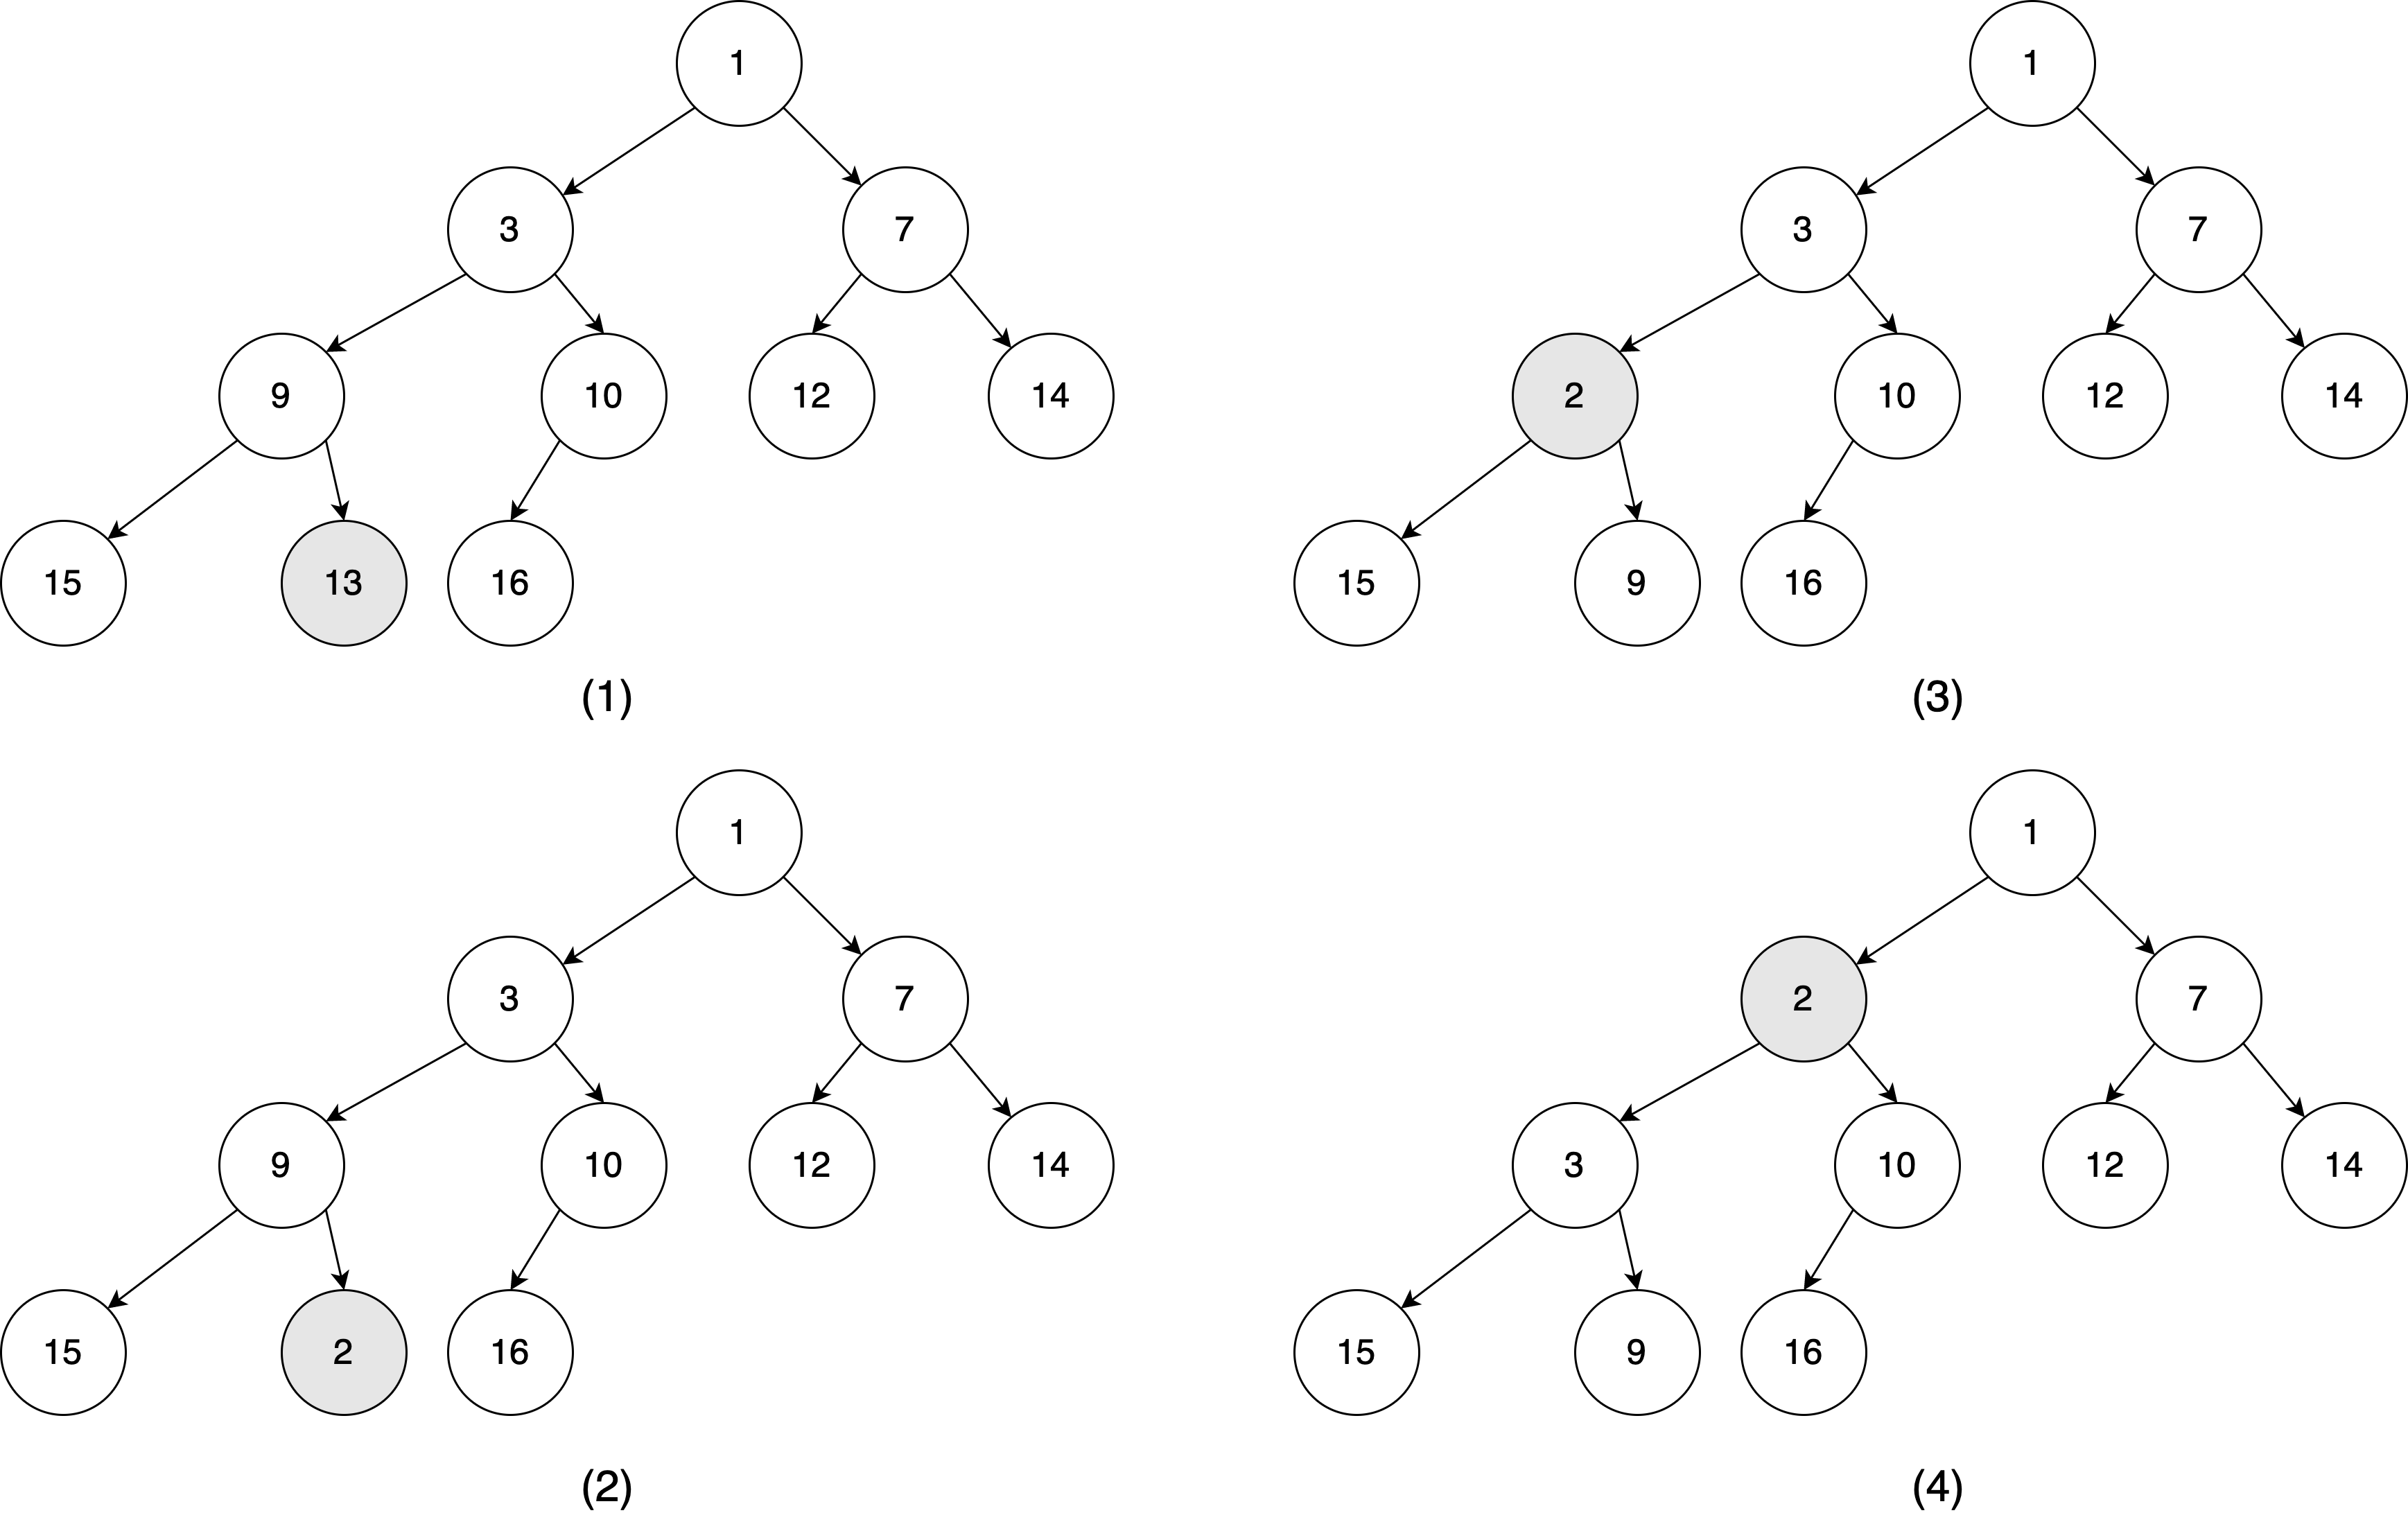
\includegraphics[scale=0.4]{img/decrease-key}
  \caption{Decrease 13 to 2. Exchange 2 and 9, then exchange with 3.}
  \label{fig:decrease-key-2}
\end{figure}

The heap property may not be satisfied when decrease some element in a min-heap. Let the decreased element indexed at $i$ in the array, below function resumes the heap property bottom-up. It is bound to $O(\lg n)$ time.

\begin{algorithmic}[1]
\Function{Heap-Fix}{$A, i$}
  \While{$i>1$ and $A[i] < A[$ \Call{Parent}{$i$} $]$}
    \State \textproc{Exchange} $A[i] \leftrightarrow A[$ \Call{Parent}{$i$} $]$
    \State $i \gets$  \Call{Parent}{$i$}
  \EndWhile
\EndFunction
\end{algorithmic}

\subsubsection{Insertion}
\index{Binary heap!insertion} \index{Binary heap!push}

We can realize push with \textproc{Heap-Fix} \cite{CLRS}. Use min-heap for example, we append the new element $k$ to the tail of the array, then apply \textproc{Heap-Fix} to recover the heap property:

\begin{algorithmic}[1]
\Function{Push}{$A, k$}
  \State \Call{Append}{$A, k$}
  \State \Call{Heap-Fix}{$A, |A|$}
\EndFunction
\end{algorithmic}

\subsection{Heap sort}
\label{heap-sort} \index{Heap sort}

We can sort elements with heap. Build a min-heap from a collection of $n$ elements, the repeatedly pop the top element to obtain the ascending result. It takes $O(n)$ time to build the heap. The pop is bound to $O(\lg n)$ time, and runs for $n$ times. Therefore, the total time is bound to $O(n \lg n)$. The space is bound to $O(n)$ as we need another list to hold the result.

\begin{algorithmic}[1]
\Function{Heap-Sort}{$A$}
  \State $R \gets [\ ]$
  \State \Call{Build-Heap}{$A$}
  \While{$A \neq [\ ]$}
    \State \textproc{Append}($R$, \Call{Pop}{$A$})
  \EndWhile
  \State \Return $R$
\EndFunction
\end{algorithmic}

Robert. W. Floyd gave a fast implementation with max-heap. The top stores the maximum one. Every time, swap the head and the tail elements in the array. After that the maximum is stored to the expected position, and the previous tail becomes the new top. We next decrease the heap size by one, and apply \textproc{Heapify} to maintain the heap property. Repeat this till the heap size decrease to one. This algorithm needn't the additional space to store the result.

\begin{algorithmic}[1]
\Function{Heap-Sort}{$A$}
  \State \Call{Build-Max-Heap}{$A$}
  \State $n \gets |A|$
  \While{$n > 1$}
    \State \textproc{Exchange} $A[1] \leftrightarrow A[n]$
    \State $n \gets n - 1$
    \State \Call{Heapify}{$A[1...n], 1$}
  \EndWhile
\EndFunction
\end{algorithmic}

\begin{Exercise}
\Question{Consider another idea about in-place heap sort: Build a min-heap from the array $A$, the first element $a_1$ is in the right position. Treat the rest $[a_2, a_3, ..., a_n]$ as the new heap, and apply \textproc{Heapify} from $a_2$. Repeat this till the last element. Is this method correct?
\begin{algorithmic}[1]
\Function{Heap-Sort}{$A$}
  \State \Call{Build-Heap}{$A$}
  \For{$i = 1$ to $n - 1$}
    \State \Call{Heapify}{$A[i ... n], 1$}
  \EndFor
\EndFunction
\end{algorithmic}
}

\Question{Similarly, can we apply \textproc{Heapify} $k$ times from left to right to get the top-$k$ elements?
\begin{algorithmic}[1]
\Function{Top-K}{$A, k$}
  \State \Call{Build-Heap}{$A$}
  \State $n \gets |A|$
  \For {$i \gets 1$ to $min(k, n)$}
    \State \Call{Heapify}{$A[i ... n], 1$}
  \EndFor
\EndFunction
\end{algorithmic}
}
\end{Exercise}

\begin{Answer}
\Question{No, it is not correct. The sub-array $[a_2, a_3, ..., a_n]$ can't map back to binary heap. It's insufficient to only apply \textproc{Heapify} from $a_2$, we need run \textproc{Build-Heap} to rebuild the heap.}
\Question{For the same reason, it does not work.}
\end{Answer}

\section{Leftist heap and skew heap}
\label{ebheap}

When implement the heap with a explicit binary tree, after pop the rot, there remain two sub-trees. Both are heaps as shown in figure \ref{fig:lvr}. How can we merge them to a new heap? To maintain the heap property, the new root must be the minimum for the remaining. We can give the first edge cases easily:

\begin{figure}[htbp]
  \centering
  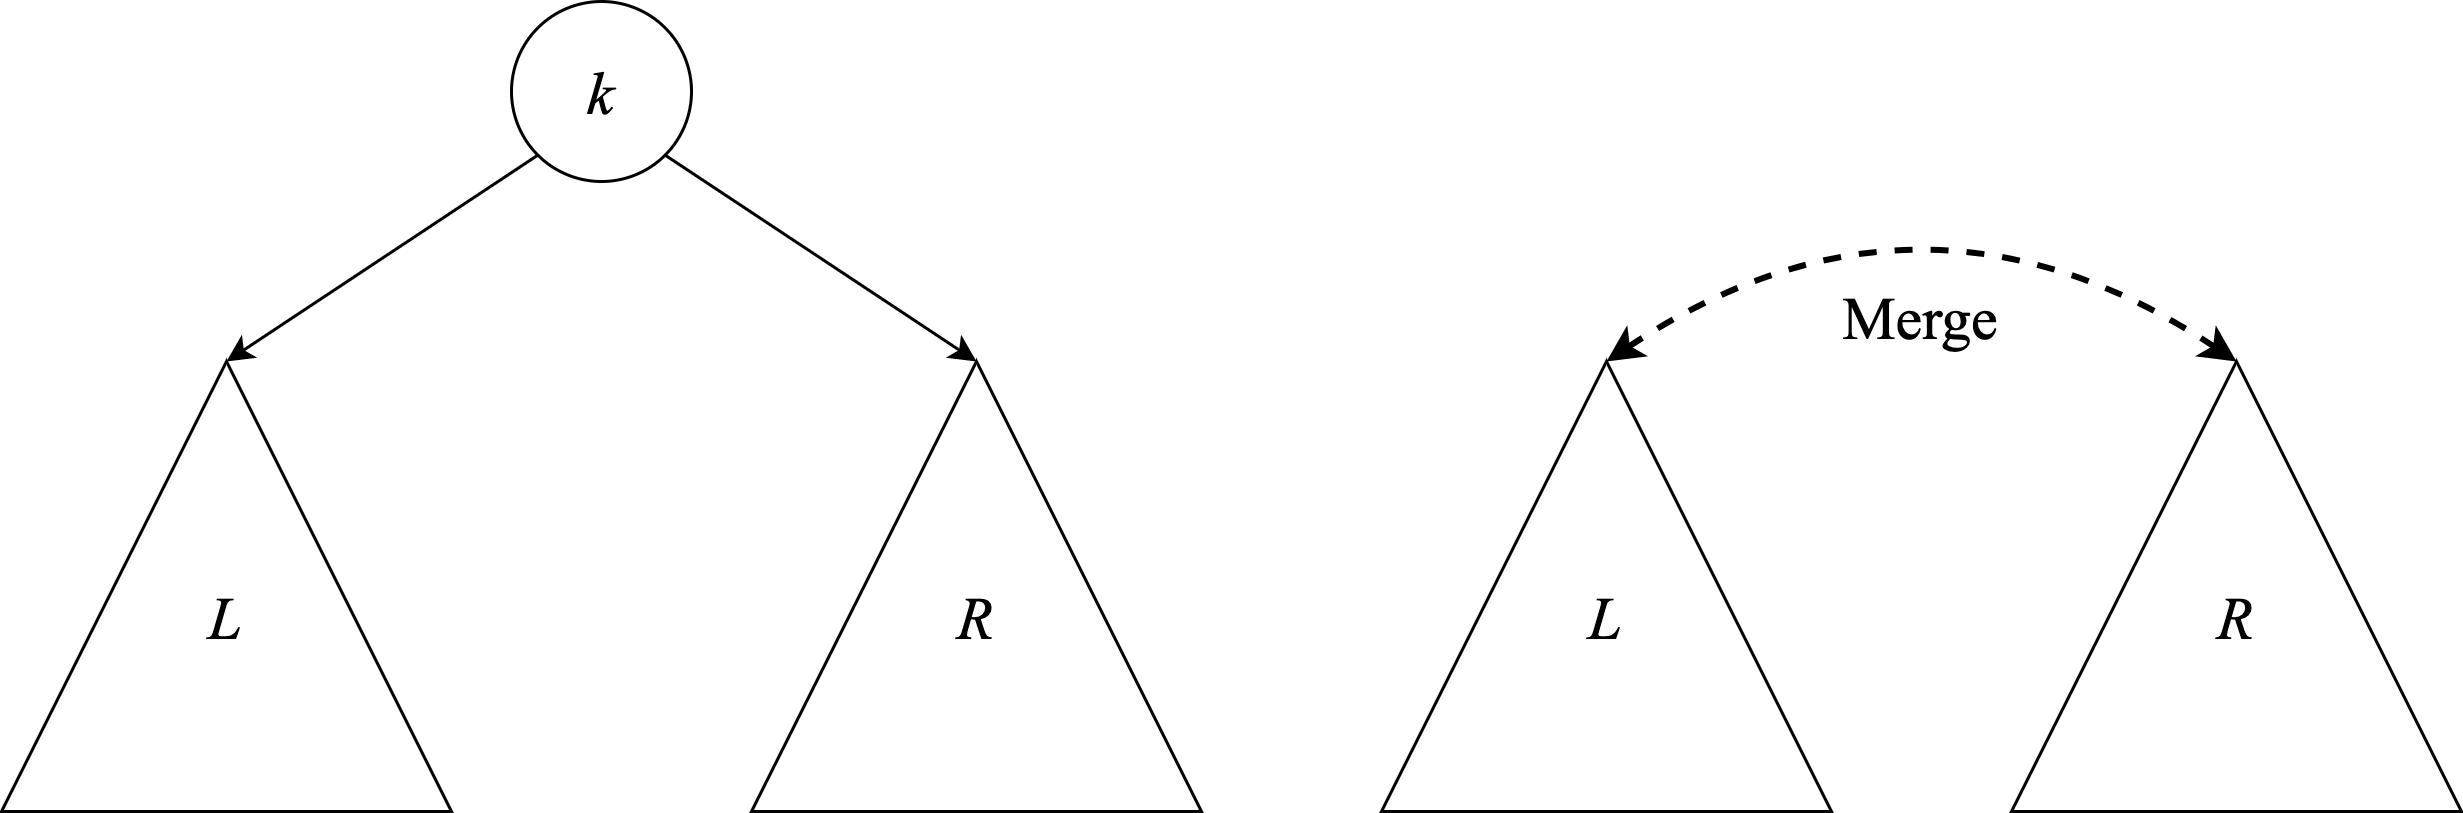
\includegraphics[scale=0.5]{img/lkr}
  \caption{Merge left and right sub-trees after pop.}
  \label{fig:lvr}
\end{figure}

\[
\begin{array}{rcl}
merge(\nil, R) & = & R \\
merge(L, \nil) & = & L \\
merge(L, R) & = & ? \\
\end{array}
\]

Both left and right sub-trees are heaps. When they are not empty, each root stores the minimum respectively. We can compare the two roots, and peek the smaller as the new root. Let $L = (A, x, B)$, $R = (A', y, B')$, where $A$, $A'$, $B$, $B'$ are sub-trees. If $x < y$, then $x$ is the new root. We keep $A$, and merge $B$ and $R$ recursively; alternatively, we can keep $B$, and merge $A$ and $R$. The new heap can be $(merge(A, R), x, B)$ or $(A, x, merge(B, R))$. Both are right. To simplify, we always merge the right sub-tree. This method generates {\em leftist heap}.

\subsection{Leftist heap}
\index{Leftist heap} \index{Leftist heap!rank} \index{Leftist heap!S-value}

The leftist heap is implemented with leftist tree. C. A. Crane in 1972\cite{wiki-leftist-tree} developed leftist tree. He defined a rank for every node (also known as $S$-value) as the distance to the nearest NIL. The rank of NIL is 0. As shown in \ref{fig:rank}, The nearest leaf node to 4 is 8, the rank of 4 is 2; Both 4 and 8 are leaves, their ranks are 1. Although the left sub-tree of 5 is not empty, its right sub-tree is NIL, hence the rank is 1. We can define the merge method with rank as below. Let the ranks for left and right sub-trees be $r_l$, $r_r$ respectively:

\begin{figure}[htbp]
  \centering
  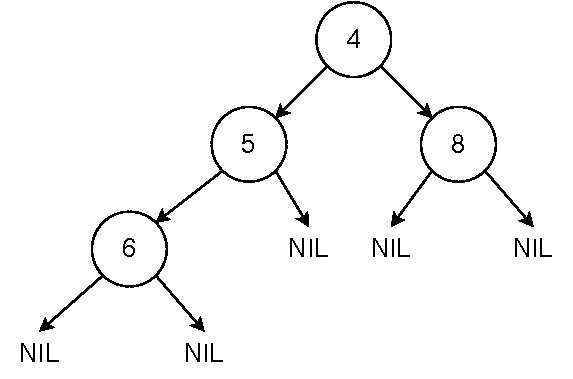
\includegraphics[scale=0.5]{img/rank}
  \caption{$rank(4) = 2$, $rank(6) = rank(8) = rank(5) = 1$.}
  \label{fig:rank}
\end{figure}

\begin{enumerate}
\item Always merge the right sub-tree;
\item When $r_l < r_r$, exchange the left and right sub-trees.
\end{enumerate}

We call above merge rules `leftist property'. Basically, a leftist tree always has the shortest path to some NIL on the right. It tends to be unbalanced, while maintain a critical constraint:

\begin{theorem}
For a leftist tree $T$ of $n$ nodes, the path from root to the rightmost NIL has at most $\lfloor \log (n + 1) \rfloor$ nodes.
\end{theorem}

We skip the proof \cite{brono-book} \cite{TAOCP}. With this theorem, algorithms process along this path are ensured bound to $O(\lg n)$ time. We can define the leftist tree by reusing binary tree plus an additional rank. Let the none empty leftist tree be $(r, L, k, R)$:

\lstset{frame = single}
\begin{Haskell}
data LHeap a = E -- Empty
             | Node Int (LHeap a) a (LHeap a)
\end{Haskell}

Function $rank$ returns the rank value:

\be
\begin{array}{rcl}
rank\ \nil & = & 0 \\
rank\ (r, L, k, R) & = & r \\
\end{array}
\ee

\subsubsection{Merge}
\index{Leftist heap!merge}

To merge two leftist heaps, we define a $make$ function. It compares the ranks of the sub-trees and swap them if necessary.

\be
make(A, k, B) = \begin{cases}
  rank(A) < rank(B) : & (rank(A) + 1, B, k, A) \\
  \text{否则}: & (rank(B) + 1, A, k, B) \\
  \end{cases}
\ee

It takes two sub-trees $A$ and $B$. If rank of $A$ is smaller, we let $B$ be the left sub-tree, and $A$ be the right. The rank of the new node is $rank(A) + 1$; otherwise if rank of $B$ is smaller, we let $A$ be the left sub-tree, and $B$ be the right. The rank of the new node is $rank(B) + 1$. Given two leftist heaps $H_1$ and $H_2$, if they are not empty, let them be $(r_1, L_1, K_1, R_1)$ and $(r_2, L_2, k_2, R_2)$ respectively. Below function defines merge:

\be
\begin{array}{rcl}
  \textit{merge}\ \nil\ H_2 & = & H_2 \\
  \textit{merge}\ H_1\ \nil & = & H_1 \\
  \textit{merge}\ H_1\ H_2 & = & \begin{cases}
  k_1 < k_2 : & make(L_1, k_1, \textit{merge}\ R_1\ H_2)  \\
  \text{否则}: & make(L_2, k_2, \textit{merge}\ H_1\ R_2) \\
  \end{cases}
\end{array}
\ee

We always apply $merge$ to the right sub-tree recursively, hence the leftist property is maintained, and it is bound to $O(\lg n)$ time.The binary heap implemented by array performs well in most cases, and it suitable for the modern cache technology. However, it takes $O(n)$ time for merge. We need concatenate two arrays, and rebuild the heap\cite{NIST}.

\begin{algorithmic}[1]
\Function{Merge-Heap}{$A, B$}
  \State $C \gets$ \Call{Concat}{$A, B$}
  \State \Call{Build-Heap}{$C$}
\EndFunction
\end{algorithmic}

We can define most heap operations with $merge$.

\subsubsection{Top and pop}
\index{Leftist heap!top} \index{Leftist heap!pop}

We can access the top element in $O(1)$ time, assume the heap is not empty:

\be
top\ (r, L, k, R) = k
\ee

After pop the root, we merge the left and right sub-trees as a new heap. Same as $merge$, pop is also bound to $O(\lg n)$ time.

\be
pop\ (r, L, k, R) = merge\ L\ R
\ee

\subsubsection{Insert}
\index{Leftist heap!insert}

To insert a new element $k$, we build a singleton leaf of $k$, then merge it with the heap:

\be
insert\ k\ H = merge\ (1, \nil, k, \nil)\ H
\ee

Or write it in Curried form as $build = fold_r\ insert\ \nil$.

\begin{figure}[htbp]
  \centering
  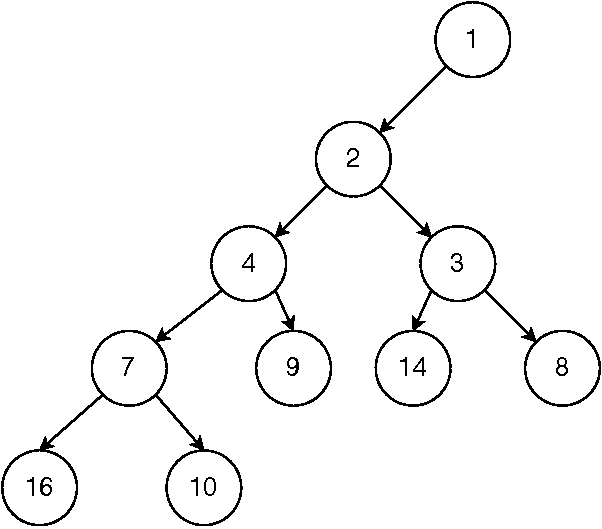
\includegraphics[scale=0.5]{img/leftist-tree}
  \caption{Build the leftist heap from $[9, 4, 16, 7, 10, 2, 14, 3, 8, 1]$.}
  \label{fig:leftist-tree}
\end{figure}

\subsubsection{Heap sort}
\index{Leftist heap!heap sort}

Given a list, we build a leftist heap from it, then repeatedly pop the minimum element from top to obtain the sorted result.

\be
sort = heapSort \circ build
\ee

Where

\be
\begin{array}{rcl}
heapSort\ [\ ] & = & [\ ] \\
heapSort\ H & = & (top\ H) : (heapSort\ (pop\ H)) \\
\end{array}
\ee

We call pop $n$ times, each takes $O(\lg n)$ time. The total time is bound to $O(n \lg n)$.

\subsection{Skew heap}
\label{skew-heap} \index{Skew heap}

Leftist heap may lead to unbalanced tree in some cases as shown in figure \ref{fig:unbalanced-leftist-tree}. Skew heap is a self-adjusting heap. It simplifies the leftist heap and improves balance\cite{wiki-skew-heap} \cite{self-adjusting-heaps}. When build the leftist heap, we swap the left and right sub-trees when the rank on left is smaller than the right. However, this method can't handle the case when either sub-tree has a NIL node. The rank is always 1 no matter how big the sub-tree is. Skew heap simplified the merge, it always swap the left and right sub-trees.

\begin{figure}[htbp]
  \centering
  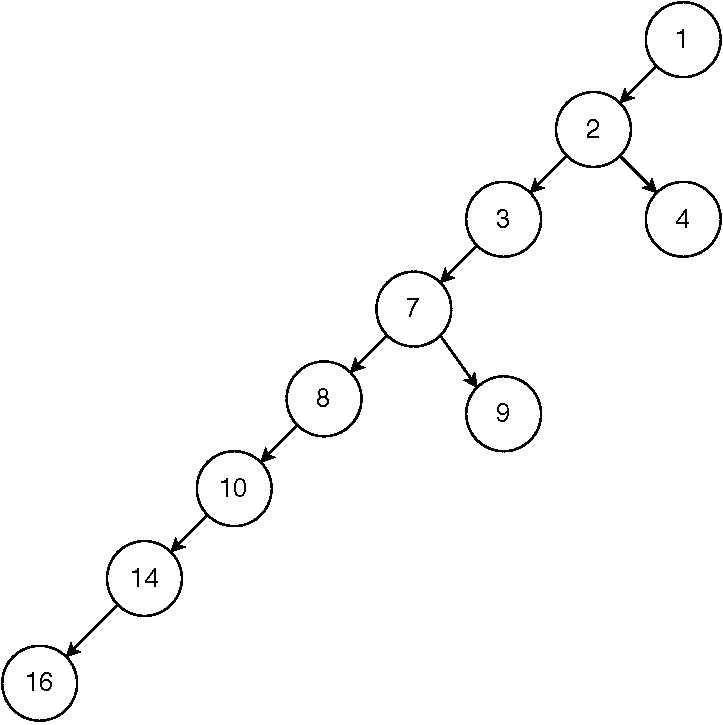
\includegraphics[scale=0.45]{img/unbalanced-leftist-tree}
  \caption{Leftist heap built from $[16, 14, 10, 8, 7, 9, 3, 2, 4, 1]$.}
  \label{fig:unbalanced-leftist-tree}
\end{figure}

Skew heap is implemented with skew tree. Skew tree is a binary tree. The root stores the minimum element, every sub-tree is also a skew tree. Skew tree needn't the rank. We can directly re-use the binary tree definition. Let the none empty tree be $(L, k, R)$.

\begin{Haskell}
data SHeap a = E -- Emtpy
             | Node (SHeap a) a (SHeap a)
\end{Haskell}

\subsubsection{Merge}
\index{Skew heap!merge} \index{Skew heap!insertion} \index{Skew heap!top} \index{Skew heap!pop}

When merge two none empty skew trees, we choose the smaller root as the new root. Then merge the greater tree with a sub-tree, and swap the left and right sub-trees. Let the two trees be $H_1 = (L_1, k_1, R_1)$ and $H_2 =(L_2, k_2, R_2)$. If $k_1 < k_2$, then choose $k_1$ as the new root. We can either merge $H_2$ with $L_1$, or merge $H_2$ with $R_1$. We choose $R_1$, and swap the left and right sub-trees. The result is $(merge(R_1, H_2), k_1, L_1)$.

\be
\begin{array}{rcl}
merge\ \nil\ H_2 & = & H_2 \\
merge\ H_1\ \nil & = & H_1 \\
merge\ H_1\ H_2\ & = & \begin{cases}
  k_1 < k_2: & (merge(R_1, H_2), k_1, L_1) \\
  \text{otherwise}: & (merge(H_1, R_2), k_2, L_2) \\
\end{cases}
\end{array}
\ee

Similar with leftist tree, the other operations, including insert, top, and pop are implemented with $merge$. Skew heap outputs a balanced tree even for ordered list as shown in figure \ref{fig:skew-tree}.

\begin{figure}[htbp]
  \centering
  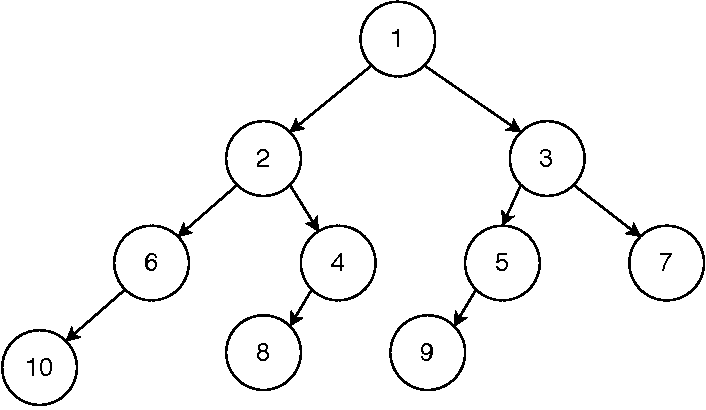
\includegraphics[scale=0.5]{img/skew-tree}
  \caption{Skew tree built from $[1, 2, ..., 10]$.}
  \label{fig:skew-tree}
\end{figure}

\section{Splay heap}
\label{splayheap} \index{Splay heap}

The leftist heap and skew heap are implemented with binary tree. If change to binary search tree, then the minimum element will not be in root. We need $O(\lg n)$ time to locate the minimum. The performance will downgrade if the tree is not balanced. Although we can use the red-black tree to secure balancing, the splay tree provides a light weight implementation. It dynamically make the tree balanced. Splay tree takes cache-like approach. It rotates the node currently being accessed to the root, reduces the access time for next visit. We define such operation as 'splay'. The tree tends to be more balanced after several splay operations. Most splay tree operations perform in amortized $O(\lg n)$ time. Daniel Dominic Sleator and Robert Endre Tarjan developed splay tree in 1985\cite{wiki-splay-tree}\cite{self-adjusting-trees}.

\subsection{Splay}
\index{Splay heap!splay}

There are two methods to do splaying. The first one need deal
with many different cases, but can be implemented fairly easy with
pattern matching. The second one has a uniformed form, but the implementation
is complex.

Denote the node currently being accessed as $X$, the parent node as $P$,
and the grand parent node as $G$ (If there are).  There are 3 steps for
splaying. Each step contains 2 symmetric cases. For illustration
purpose, only one case is shown for each step.

\begin{itemize}
\item {\em Zig-zig step.} As shown in figure \ref{fig:zig-zig}, in this case,
$X$ and $P$ are children on the same side of $G$, either both on left or right. By
rotating 2 times, $X$ becomes the new root.

\begin{figure}[htbp]
  \centering
  \subcaptionbox{$X$ and $P$ are both left children or both right children.}{\includegraphics[scale=0.4]{img/zig-zig-a}}
  \subcaptionbox{$X$ becomes new root after rotating 2 times.}{\includegraphics[scale=0.4]{img/zig-zig-b}}
  \caption{Zig-zig case.} \label{fig:zig-zig}
\end{figure}

\item {\em Zig-zag step.} As shown in figure \ref{fig:zig-zag}, in this
case, $X$ and $P$ are children on different sides. $X$ is on the left,
$P$ is on the right. Or $X$ is on the right, $P$ is on the left.
After rotation, $X$ becomes the new root, $P$ and $G$ are siblings.

\begin{figure}[htbp]
  \centering
  \subcaptionbox{$X$ and $P$ are children on different sides.}{\includegraphics[scale=0.4]{img/zig-zag-a}}
  \subcaptionbox{$X$ becomes new root. $P$ and $G$ are siblings.}{\includegraphics[scale=0.4]{img/zig-zag-b}}
  \caption{Zig-zag case.} \label{fig:zig-zag}
\end{figure}

\item {\em Zig step.} As shown in figure \ref{fig:zig}, in this case,
$P$ is the root, we rotate the tree, so that $X$ becomes new root.
This is the last step in splay operation.

\begin{figure}[htbp]
  \centering
  \subcaptionbox{$P$ is the root.}{\includegraphics[scale=0.4]{img/zig-a}}
  \subcaptionbox{Rotate the tree to make $X$ be new root.}{\includegraphics[scale=0.4]{img/zig-b}}
  \caption{Zig case.} \label{fig:zig}
\end{figure}

\end{itemize}

Although there are 6 different cases, they can be handled in the
environments support pattern matching. Denote the non-empty binary tree
in form $T=(L, k, R)$,. when access key $Y$ in tree $T$, the splay
operation can be defined as below.

\be
splay(T, X) = \left \{
  \begin{array}
  {r@{\quad:\quad}l}
  (a, X, (b, P, (c, G, d))) & T = (((a, X, b), P, c), G, d), X = Y \\
  (((a, G, b), P, c), X, d) & T= (a, G, (b, P, (c, X, d))), X = Y \\
  ((a, P, b), X, (c, G, d)) & T = (a, P, (b, X, c), G, d), X = Y \\
  ((a, G, b), X, (c, P, d)) & T = (a, G, ((b, X, c), P, d)), X = Y \\
  (a, X, (b, P, c)) & T = ((a, X, b), P, c), X = Y \\
  ((a, P, b), X, c) & T = (a, P, (b, X, c)), X = Y \\
  T &  otherwise
  \end{array}
\right.
\ee

The first two clauses handle the 'zig-zig' cases; the next two
clauses handle the 'zig-zag' cases; the last two clauses handle
the zig cases. The tree aren't changed for all other situations.

The following Haskell program implements this splay function.

\lstset{language=Haskell}
\begin{lstlisting}
data STree a = E -- Empty
             | Node (STree a) a (STree a) -- left, key, right

-- zig-zig
splay t@(Node (Node (Node a x b) p c) g d) y =
    if x == y then Node a x (Node b p (Node c g d)) else t
splay t@(Node a g (Node b p (Node c x d))) y =
    if x == y then Node (Node (Node a g b) p c) x d else t
-- zig-zag
splay t@(Node (Node a p (Node b x c)) g d) y =
    if x == y then Node (Node a p b) x (Node c g d) else t
splay t@(Node a g (Node (Node b x c) p d)) y =
    if x == y then Node (Node a g b) x (Node c p d) else t
-- zig
splay t@(Node (Node a x b) p c) y = if x == y then Node a x (Node b p c) else t
splay t@(Node a p (Node b x c)) y = if x == y then Node (Node a p b) x c else t
-- otherwise
splay t _ = t
\end{lstlisting}

With splay operation defined, every time when insert a new key,
we call the splay function to adjust the tree.
If the tree is empty, the result is a leaf; otherwise we compare this key
with the root, if it is less than the root, we recursively insert it into
the left child, and perform splaying after that; else the key is inserted
into the right child.

\be
insert(T, x) = \left \{
  \begin{array}
  {r@{\quad:\quad}l}
  (\phi, x, \phi) & T = \phi \\
  splay((insert(L, x), k, R), x) & T = (L, k, R), x < k \\
  splay(L, k, insert(R, x)) & otherwise
  \end{array}
  \right.
\ee

The following Haskell program implements this insertion algorithm.

\lstset{language=Haskell}
\begin{lstlisting}
insert E y = Node E y E
insert (Node l x r) y
    | x > y     = splay (Node (insert l y) x r) y
    | otherwise = splay (Node l x (insert r y)) y
\end{lstlisting}

Figure \ref{fig:splay-result} shows the result of using this function.
It inserts the ordered elements $\{1, 2, ..., 10\}$
one by one to the empty tree. This would build a very poor result
which downgrade to linked-list with normal binary search tree.
The splay method creates more balanced result.

\begin{figure}[htbp]
  \centering
  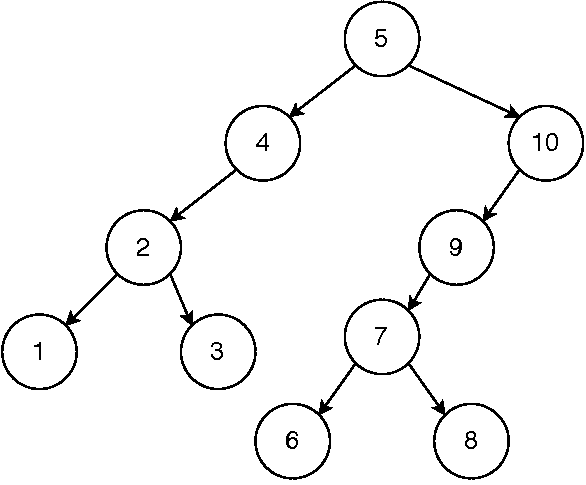
\includegraphics[scale=0.5]{img/splay-tree}
  \caption{Splaying helps improving the balance.}
  \label{fig:splay-result}
\end{figure}

Okasaki found a simple rule for Splaying \cite{okasaki-book}.
Whenever we follow
two left branches, or two right branches continuously, we rotate
the two nodes.

Based on this rule, splaying can be realized in such a way.
When we access node for a key $x$ (can be during the process of
inserting a node, or looking up a node, or deleting a node), if
we traverse two left branches or two right branches, we
partition the tree in two parts $L$ and $R$, where $L$ contains all
nodes smaller than $x$, and $R$ contains all the rest.
We can then create a new tree (for instance in insertion),
with $x$ as the root, $L$ as the left child, and $R$ being the right child.
The partition process is recursive, because it will splay
its children as well.

\be
partition(T, p) = \left \{
  \begin{array}
  {r@{\quad:\quad}l}
  (\phi, \phi) & T = \phi \\
  (T, \phi) & T = (L, k, R) \land R = \phi \\
  ((L, k, L'), k', A, B) & \begin{array}{l} \\
                             T = (L, k, (L', k', R')) \\
                             k < p, k' < p \\
                             (A, B) = partition(R', p)
                           \end{array} \\
  ((L, k, A), (B, k', R')) & \begin{array}{l} \\
                               T = (L, K, (L', k', R')) \\
                               k < p \leq k' \\
                               (A, B) = partition(L', p) \\ \\
                             \end{array} \\
  (\phi, T) & T = (L, k, R) \land L = \phi \\
  (A, (L', k', (R', k, R)) & \begin{array}{l} \\
                               T = ((L', k', R'), k, R) \\
                               p \leq k, p \leq k' \\
                               (A, B) = partition(L', p)
                             \end{array} \\
  ((L', k', A), (B, k, R)) & \begin{array}{l} \\
                               T = ((L', k', R'), k, R) \\
                               k' \leq p \leq k \\
                               (A, B) = partition(R', p)
                             \end{array}
  \end{array}
  \right.
\ee

Function $partition(T, p)$ takes a tree $T$, and a pivot $p$ as arguments.
The first clause is edge case. The partition result for empty is
a pair of empty left and right trees. Otherwise, denote the tree
as $(L, k, R)$. we need compare the pivot $p$ and the root $k$.
If $k < p$, there are two sub-cases. one is trivial case that
$R$ is empty. According to the property of binary search tree,
All elements are less than $p$, so the result pair is $(T, \phi)$;
For the other case, $R = (L', k', R')$, we need further compare
$k'$ with the pivot $p$. If $k' < p$ is also true, we recursively
partition $R'$ with the pivot, all the elements less than $p$ in
$R'$ is held in tree $A$, and the rest is in tree $B$. The
result pair can be composed with two trees, one is $((L, k, L'), k', A)$;
the other is $B$. If the key of the right sub tree is not less than
the pivot, we recursively partition $L'$ with the pivot to give
the intermediate pair $(A, B)$, the final pair trees can be
composed with $(L, k, A)$ and $(B, k', R')$. There are symmetric
cases for $p \leq k$. They are handled in the last three clauses.

Translating the above algorithm into Haskell yields the following partition
program.

\begin{lstlisting}
partition E _ = (E, E)
partition t@(Node l x r) y
    | x < y =
        case r of
          E -> (t, E)
          Node l' x' r' ->
              if x' < y then
                  let (small, big) = partition r' y in
                  (Node (Node l x l') x' small, big)
              else
                  let (small, big) = partition l' y in
                  (Node l x small, Node big x' r')
    | otherwise =
        case l of
          E -> (E, t)
          Node l' x' r' ->
              if y < x' then
                  let (small, big) = partition l' y in
                  (small, Node l' x' (Node r' x r))
              else
                  let (small, big) = partition r' y in
                  (Node l' x' small, Node big x r)
\end{lstlisting}

% ================================================================
%                 Basic heap operations
% ================================================================
\index{Splay heap!insertion}
Alternatively, insertion can be realized with $partition$ algorithm.
When insert a new element $k$ into
the splay heap $T$, we can first partition the heap into two trees, $L$ and $R$. Where
$L$ contains all nodes smaller than $k$, and $R$ contains the rest.
We then construct a new node, with $k$ as the root and $L$, $R$ as the children.

\be
insert(T, k) = (L, k, R), (L, R) = partition(T, k)
\ee

The corresponding Haskell example program is as the following.

\lstset{language=Haskell}
\begin{lstlisting}
insert t x = Node small x big where (small, big) = partition t x
\end{lstlisting}

\subsubsection{Top and pop}
\index{Splay heap!top}
\index{Splay heap!pop}
Since splay tree is just a special binary search tree, the minimum
element is stored in the left most node. We need keep traversing
the left child to realize the top operation. Denote the none empty
tree $T=(L, k, R)$, the $top(T)$ function can be defined as below.

\be
top(T) = \left \{
  \begin{array}
  {r@{\quad:\quad}l}
  k & L = \phi \\
  top(L) & otherwise
  \end{array}
  \right.
\ee

This is exactly the $min(T)$ algorithm for binary search tree.

For pop operation, the algorithm need remove the minimum element from the
tree. Whenever there
are two left nodes traversed, the splaying operation should be performed.

\be
pop(T) = \left \{
  \begin{array}
  {r@{\quad:\quad}l}
  R & T = (\phi, k, R) \\
  (R', k, R) & T = ((\phi, k', R'), k, R) \\
  (pop(L'), k', (R', k, R)) & T = ((L', k', R'), k, R)
  \end{array}
  \right.
\ee

Note that the third clause performs splaying without explicitly call
the $partition$ function. It utilizes the property of binary
search tree directly.

Both the top and pop algorithms are bound to $O(\lg n)$ time because
the splay tree is balanced.

The following Haskell example programs implement the top and pop
operations.

\lstset{language=Haskell}
\begin{lstlisting}
findMin (Node E x _) = x
findMin (Node l x _) = findMin l

deleteMin (Node E x r) = r
deleteMin (Node (Node E x' r') x r) = Node r' x r
deleteMin (Node (Node l' x' r') x r) = Node (deleteMin l') x' (Node r' x r)
\end{lstlisting}

\subsubsection{Merge}
\index{Splay heap!merge}
Merge is another basic operation for heaps as it is widely used in Graph algorithms. By using the $partition$ algorithm, merge can be realized in $O(\lg n)$ time.

When merging two splay trees, for non-trivial case, we can take the root of the first tree as the new root, then partition the second tree with this new root as the pivot. After that we recursively merge
the children of the first tree to the partition result. This algorithm is defined as the following.

\be
merge(T_1, T_2) = \left \{
  \begin{array}
  {r@{\quad:\quad}l}
  T_2 & T_1 = \phi \\
  (merge(L, A), k, merge(R, B)) & T_1 = (L, k, R), (A, B) = partition(T_2, k)
  \end{array}
  \right.
\ee

If the first heap is empty, the result is definitely the second heap. Otherwise,
denote the first splay heap as $(L, k, R)$, we partition $T_2$ with $k$ as the
pivot to yield $(A, B)$, where $A$ contains all the elements in $T_2$ which are
less than $k$, and $B$ holds the rest. We next recursively merge $A$ with $L$;
and merge $B$ with $R$ as the new children for $T_1$.

Translating the definition to Haskell gives the following example program.

\lstset{language=Haskell}
\begin{lstlisting}
merge E t = t
merge (Node l x r) t = Node (merge l l') x (merge r r')
    where (l', r') = partition t x
\end{lstlisting}

% ================================================================
%                 Heap sort
% ================================================================
\subsection{Heap sort}

Since the internal implementation of the Splay heap is completely
transparent to the heap interface, the heap sort algorithm can
be reused. It means that the heap sort algorithm is generic no
matter what the underground data structure is.

% ================================================================
%                 Short summary
% ================================================================
\section{Notes and short summary}

In this chapter, we define binary heap more general
so that as long as the heap property is maintained, all binary
representation of data structures can be used to implement binary heap.

This definition doesn't limit to the popular array based binary
heap, but also extends to the explicit binary heaps including Leftist
heap, Skew heap and Splay heap. The array based binary heap
is particularly convenient for the imperative implementation
because it intensely uses random index access which can be mapped to
a completely binary tree. It's hard to find directly functional
counterpart in this way.

However, by using explicit binary tree, functional implementation
can be achieved, most of them have $O(\lg n)$ worst case
performance, and some of them even reach $O(1)$ amortize time.
Okasaki in \cite{okasaki-book} shows detailed analysis of these data
structures.

In this chapter, only purely functional realization for Leftist heap,
Skew heap, and Splay heap are explained, they can all be realized
in imperative approaches.

It's very natural to extend the concept from binary tree to
$k$-ary ($k$-way) tree, which leads to other useful heaps such as
Binomial heap, Fibonacci heap and pairing heap. They are introduced
in the following chapters.

% ================================================================
%                 Exercise
% ================================================================
\begin{Exercise}
\begin{itemize}
\item Realize the imperative Leftist heap, Skew heap, and Splay heap.
\end{itemize}
\end{Exercise}

\section{Appendix - example programs}

For the complete binary tree represented by array, access parent, and sub-trees with bit-wise operation (index from 0):

\begin{lstlisting}[language = Bourbaki]
Int parent(Int i) = ((i + 1) >> 1) - 1

Int left(Int i) = (i << 1) + 1

Int right(Int i) = (i + 1) << 1
\end{lstlisting}

Heapify, parameterized the comparison:

\begin{lstlisting}[language = Bourbaki]
void heapify([K] a, Int i, Less<K> lt) {
    Int l, r, m
    Int n = length(a)
    loop {
        m = i
        l = left(i)
        r = right(i)
        if l < n and lt(a[l], a[i]) then m = l
        if r < n and lt(a[r], a[m]) then m = r
        if m != i {
            swap(a, i, m);
            i = m
        } else {
            break
        }
    }
}
\end{lstlisting}

Build the binary heap from array:

\begin{lstlisting}[language = Bourbaki]
void buildHeap([K] a, Less<K> lt) {
    Int n = length(a)
    for Int i = (n-1) / 2 downto 0 {
        heapify(a, i, lt)
    }
}
\end{lstlisting}

Pop:

\begin{lstlisting}[language = Bourbaki]
K pop([K] a, Less<K> lt) {
    var n = length(a)
    t = a[n]
    swap(a, 0, n - 1)
    remove(a, n - 1)
    if a != [] then heapify(a, 0, lt)
    return t
}
\end{lstlisting}

Obtain the top-$k$ elements:

\begin{lstlisting}[language = Bourbaki]
[K] topk([K] a, Int k, Less<K> lt) {
    buildHeap(a, lt)
    [K] r = []
    loop min(k, length(a)) {
        append(r, pop(a, lt))
    }
    return r
}
\end{lstlisting}

Decrease the key in min-heap:

\begin{lstlisting}[language = Bourbaki]
void decreaseKey([K] a, Int i, K k, Less<K> lt) {
    if lt(k, a[i]) {
        a[i] = k
        heapFix(a, i, lt)
    }
}

void heapFix([K] a, Int i, Less<K> lt) {
    while i > 0 and lt(a[i], a[parent(i)]) {
        swap(a, i, parent(i))
        i = parent(i)
    }
}
\end{lstlisting}

Push new element:

\begin{lstlisting}[language = Bourbaki]
void push([K] a, K k, less<K> lt) {
    append(a, k)
    heapFix(a, length(a) - 1, lt)
}
\end{lstlisting}

Heap sort:

\begin{lstlisting}[language = Bourbaki]
void heapSort([K] a, less<K> lt) {
    buildHeap(a, not . lt)
    n = length(a)
    while n > 1 {
        swap(a, 0, n - 1)
        n = n - 1
        heapify(a[0 .. (n - 1)], 0, not . lt)
    }
}
\end{lstlisting}

Merge two leftist heaps:

\begin{Haskell}
merge E h = h
merge h E = h
merge h1@(Node _ x l r) h2@(Node _ y l' r') =
    if x < y then makeNode x l (merge r h2)
    else makeNode y l' (merge h1 r')

makeNode x a b = if rank a < rank b then Node (rank a + 1) x b a
                 else Node (rank b + 1) x a b
\end{Haskell}

Merge two skew heaps:

\begin{Haskell}
merge E h = h
merge h E = h
merge h1@(Node x l r) h2@(Node y l' r') =
    if x < y then Node x (merge r h2) l
    else Node y (merge h1 r') l'
\end{Haskell}

Splay operation:

\begin{Haskell}
-- zig-zig
splay t@(Node (Node (Node a x b) p c) g d) y =
    if x == y then Node a x (Node b p (Node c g d)) else t
splay t@(Node a g (Node b p (Node c x d))) y =
    if x == y then Node (Node (Node a g b) p c) x d else t
-- zig-zag
splay t@(Node (Node a p (Node b x c)) g d) y =
    if x == y then Node (Node a p b) x (Node c g d) else t
splay t@(Node a g (Node (Node b x c) p d)) y =
    if x == y then Node (Node a g b) x (Node c p d) else t
-- zig
splay t@(Node (Node a x b) p c) y = if x == y then Node a x (Node b p c) else t
splay t@(Node a p (Node b x c)) y = if x == y then Node (Node a p b) x c else t
-- 否则
splay t _ = t
\end{Haskell}

Insert new element to the splay heap:

\begin{Haskell}
insert E y = Node E y E
insert (Node l x r) y
    | x > y     = splay (Node (insert l y) x r) y
    | otherwise = splay (Node l x (insert r y)) y
\end{Haskell}

Partition the splay tree:

\begin{Haskell}
partition E _ = (E, E)
partition t@(Node l x r) y
    | x < y =
        case r of
          E -> (t, E)
          Node l' x' r' ->
              if x' < y then
                  let (small, big) = partition r' y in
                  (Node (Node l x l') x' small, big)
              else
                  let (small, big) = partition l' y in
                  (Node l x small, Node big x' r')
    | otherwise =
        case l of
          E -> (E, t)
          Node l' x' r' ->
              if y < x' then
                  let (small, big) = partition l' y in
                  (small, Node l' x' (Node r' x r))
              else
                  let (small, big) = partition r' y in
                  (Node l' x' small, Node big x r)
\end{Haskell}

Merge two splay trees:

\begin{Haskell}
merge E t = t
merge (Node l x r) t = Node (merge l l') x (merge r r')
    where (l', r') = partition t x
\end{Haskell}

\ifx\wholebook\relax \else
\section{Answers}
\shipoutAnswer

\begin{thebibliography}{99}

\bibitem{CLRS}
Thomas H. Cormen, Charles E. Leiserson, Ronald L. Rivest and Clifford Stein. ``Introduction to Algorithms, Second Edition''. The MIT Press, 2001. ISBN: 0262032937.

\bibitem{wiki-heap}
Heap (data structure), Wikipedia. \url{https://en.wikipedia.org/wiki/Heap_(data_structure)}

\bibitem{wiki-heapsort}
Heapsort, Wikipedia. \url{https://en.wikipedia.org/wiki/Heapsort}

\bibitem{okasaki-book}
Chris Okasaki. ``Purely Functional Data Structures''. Cambridge university press, (July 1, 1999), ISBN-13: 978-0521663502

\bibitem{rosetta-heapsort}
Sorting algorithms/Heapsort. Rosetta Code. \url{http://rosettacode.org/wiki/Sorting_algorithms/Heapsort}

\bibitem{wiki-leftist-tree}
Leftist Tree, Wikipedia. \url{https://en.wikipedia.org/wiki/Leftist_tree}

\bibitem{brono-book}
Bruno R. Preiss. Data Structures and Algorithms with Object-Oriented Design Patterns in Java. \url{http://www.brpreiss.com/books/opus5/index.html}

\bibitem{TAOCP}
Donald E. Knuth. ``The Art of Computer Programming. Volume 3: Sorting and Searching.''. Addison-Wesley Professional;
2nd Edition (October 15, 1998). ISBN-13: 978-0201485417. Section 5.2.3 and 6.2.3

\bibitem{wiki-skew-heap}
Skew heap, Wikipedia. \url{https://en.wikipedia.org/wiki/Skew_heap}

\bibitem{self-adjusting-heaps}
Sleator, Daniel Dominic; Jarjan, Robert Endre. ``Self-adjusting heaps'' SIAM Journal on Computing 15(1):52-69. doi:10.1137/0215004 ISSN 00975397 (1986)

\bibitem{wiki-splay-tree}
Splay tree, Wikipedia. \url{https://en.wikipedia.org/wiki/Splay_tree}

\bibitem{self-adjusting-trees}
Sleator, Daniel D.; Tarjan, Robert E. (1985), ``Self-Adjusting Binary Search Trees'', Journal of the ACM 32(3):652 - 686, doi: 10.1145/3828.3835

\bibitem{NIST}
NIST, ``binary heap''. \url{http://xw2k.nist.gov/dads//HTML/binaryheap.html}

\end{thebibliography}

\expandafter\enddocument
\fi
